\chapter{Problem Analysis}

In this chapter, we will discuss the decisions we made during application design and reasons behind every choice. We will define what influenced the chosen application structure. Finally, we will explain the purpose of each part of the application.

%%-----------------------------------------------------------------------------------------
%% SECTION
%%-----------------------------------------------------------------------------------------
\section{Design Guidelines}
At the beginning of the design we decided to establish three main design guidelines that would help us create a successful application:
\begin{itemize}
    \item Multi-platform application
    \item Modular design
    \item Scalability
\end{itemize}
Each of them should give us an advantage over current or future competition as well as reduce the amount of work needed compared to establishing them in the later parts of design and development.

%%-----------------------------------------------------------------------------------------
\subsection{Multi-platform Application}

First step on the way to create any piece of software is to select target platform. There are three main platforms, Windows by Microsoft leading the market share with a big margin to OS X by Apple then followed by Linux (see Fig. \ref{fig01:osMarketShareChart}).

\begin{figure}[ht]\centering
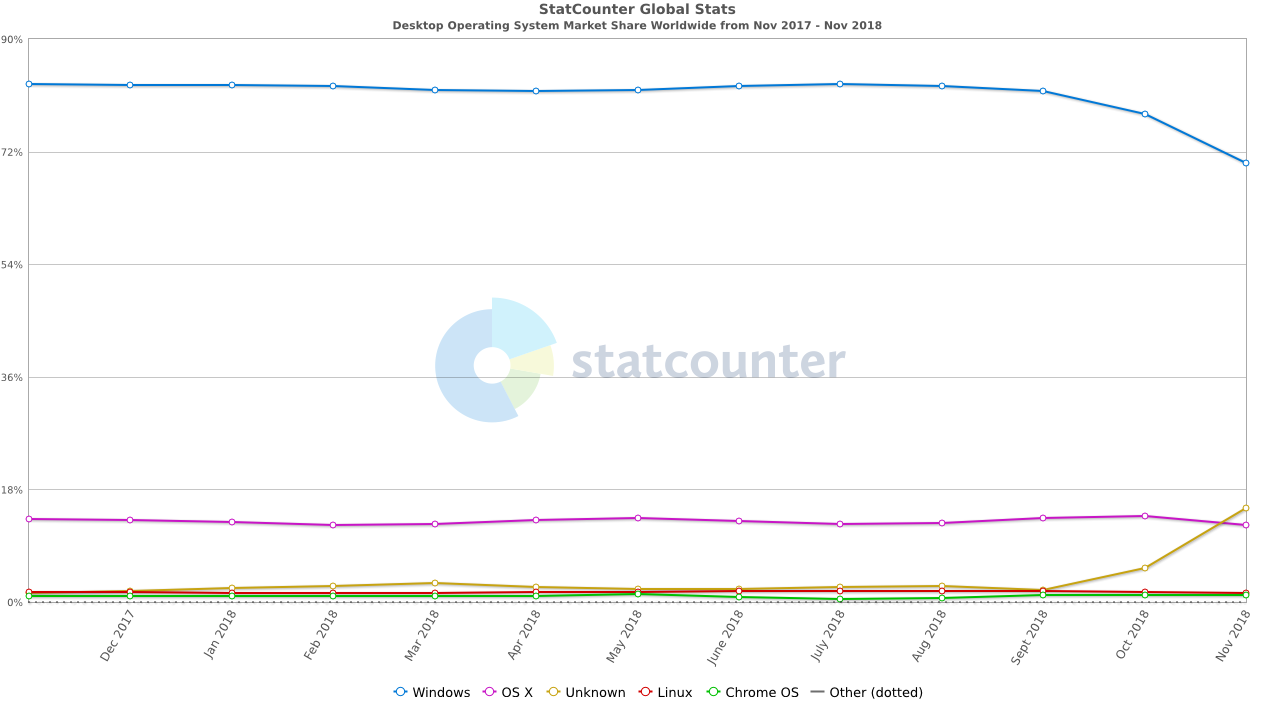
\includegraphics[width=1.0\textwidth]{img/StatCounter-os_combined-ww-monthly-201711-201811}
\caption{Desktop Operating System Market Share Worldwide from Nov 2017 - Nov 2018~\citep{osMarketShare}}
\label{fig01:osMarketShareChart}
\end{figure}

For simplicity we could assume that vast majority of users use Windows and we could target this single platform without losing many potential users. But we do not know the exact market share in our target group and focusing on single platform may be a major mistake.
\par
Another reason to support multiple platforms is the recent progress of miniature PCs. The most important task of our application is to play music and these computers have enough computing power to do that and require just a small initial investment into hardware that would do so. These PCs usually run or at least support some versions of Linux, which has the smallest market share among major operating systems.
\par
The downside compared to creating platform-specific application is some extra amount of work that needs to be done both during analysis and subsequent implementation. However, we consider the benefits of adopting this approach early to be significant enough compared to the risk of having to support additional platform after the implementation is finished.
%%-----------------------------------------------------------------------------------------
\subsection{Modular Design}

If we could divide our application into reasonable amount of modules and define exact interface and relationship among them, the resulting design would have a lot of flexibility both from user's and developer's point of view.
\par
As developers, we would be able to make best decisions regarding each module without having to worry about other modules as long as we keep the predefined interface. We can create specialized versions of one module without having to modify any other. Furthermore, no two modules have to run on the same machine, in the same building or even the same country.
\par
Instead of having one monolithic application, our users may select suitable modules and customize it to suit their needs. Every use case has its specifics and adopting this feature allows us to offer each user a suitable solution.
\par
Being bound by predefined interfaces is a drawback that we must face, so they must be designed with extra care and robustness in order to be beneficial.

\subsubsection{Splitting Functionality Into Modules}
To determine the suitability of modular design, first we need to understand what functionality our application requires. Then we can group similar functionality together and wrap it up in modules. Each module should be able to perform its task without the help of another and offer certain services to other modules or be able to consume other module's services if needed. These services will then be predefined by a certain interface so we gain an ability to work with different implementations of one module without the need to modify other modules.

\par
Below is a list of modules with a description of functionality that they offer:
\begin{itemize}
    \item Fileserver module - has access to a collection of music files. It keeps information about their location in file system. It stores their metadata like title, artist and album name. It provides the ability to browse its music library and to group songs into playlists.
    \item Player module - can play music files. In order to do that, first we need to decode them, as most music files are encoded to use less storage space. Then we can send the data to sound card to finally play some music. It also takes care of caching music files if it utilizes Fileserver module running on different machine.
    \item Manager module - provides the user interface for the application. It allows users to browse the music library and create their playlists. It gives them control over music playback. It allows them to customize the application and set the settings they need. It shows them what regular users ordered to be played.
    \item Database module - is a tool for synchronization between the application and regular users. They want to see what songs are offered in playlists and the application needs to know their orders so it can play what they desire. It also stores user account data.
\end{itemize}
Above-mentioned enumeration of functionality roughly describes requirements for each module. Since there are much more details about each of them, we will define the requirements and interface for each module later in this chapter.

%%-----------------------------------------------------------------------------------------
\subsection{Scalability}

The last fundamental feature is scalability. We have set a goal to attract a wide range of users, so our application must be able to function properly with any size of music library and any number of regular users wanting to listen to their favourite song. Having adopted modular design earlier, we can achieve scalability also by offering a more capable module as a replacement for one that has reached its maximum potential. Nevertheless, all modules should only be limited by computing power provided by the user.

%%-----------------------------------------------------------------------------------------
%% SECTION
%%-----------------------------------------------------------------------------------------
\section{Fileserver Module}

Fileserver module manages music files contained in music library. It knows the location of these files and how to access them, allows adding or removing files and distributes them on demand for playback.
\par
Fileserver handles extraction of metadata from music files. Supported metadata are song title, artist name, album name, genre name and song duration. These are stored for easier browsing of the library.
\par
This module allows to browse, search and order songs in its music library. Additionally, these songs can then be grouped in playlists. A playlist is a collection of songs from music library of the respective fileserver. It has a name and optionally a description. Every user can see only their playlists.
\par
Services provided by this module are available through a predefined interface and it does not use or require any other module.

%%-----------------------------------------------------------------------------------------
\subsection{Interface}

This interface defines how to access and browse music library offered by fileserver. We decided to support only browsing the library and managing playlists and omit manipulation with music files from this interface, as the way of working with files may differ greatly across platforms and it might also be unwanted to offer file management capability to users. Instead, implementations of this module are free to offer their own way of managing the contents of the library.
\par
First, we need to choose a suitable interface technology. We need to support distributed architecture, so we have to choose from network technologies.
\par
One option would be to communicate with fileserver over a dedicated socket. However, we declined this option, because we do not need to have an open connection with fileserver at all times so it would be a waste of resources. It would limit the number of possible connections to a fileserver and therefore the solution would not be scalable enough.
\par
Since we are dealing with sharing and transferring files over network, it would make sense to utilize one of network protocols designed for that, such as File Transfer Protocol (FTP) or Network File System (NFS) protocol. These protocols can be useful for small-scale private file servers as they can provide direct control over available files, less so for larger-scale public file servers. However, they would not provide enough abstraction that we would like to gain form this module. The benefit of this module should be to provide access to a collection of songs rather than a collection of files. Using such protocol would demand consumers of interface to maintain some file browsing capability. Nevertheless, these protocols still might be utilized in implementations for file management.
\par
Another option is to create this interface as web API. This approach seems more suitable for the task as the main purpose of the interface of fileserver is to provide access to data. While the same result can be achieved using either SOAP or REST protocols, we opted for RESTful API, because it is more modern, it is easier to implement and it uses HTTP protocol in a more straight-forward way, so the resulting implementations can be more lightweight. Furthermore, it is possible to wrap such API with GraphQL, which has recently risen in popularity since its introduction in 2015.
\par
The resulting interface follows principles of REST API design. All requests are stateless, no state needs to be stored by the interface implementation. Each resource is defined by the link that it can be accessed by and query parameters are used to modify the result. HTTP request method determines the action performed when accessing a resource. GET method is used to retrieve resources, POST method is used to create new resource, PUT requests modify resources and DELETE method removes resources. JSON file format is used for transferring data. For more details see the interface documentation \todo{add link to documentation}.

%%-----------------------------------------------------------------------------------------
%% SECTION
%%-----------------------------------------------------------------------------------------
\section {Player Module}

Player module, as its name suggests, takes care of playing music and all related tasks, such as decoding and playback control. Since music files do not have to be located on the machine where this module is running, it has to take care of getting and caching necessary music files.
\par
This module utilizes fileserver module to get music files and offers a communication channel to control its behavior.

%%-----------------------------------------------------------------------------------------
\subsection{Interface}

The behavior and consequently the interface of player module are different from fileserver module. Fileserver is stateless, can support multiple users and communication is mostly one-way. On the other hand, player needs to preserve its state, e.g. playback progress or cache, it can only support one user as there is usually only one audio device available and it needs to communicate both ways, besides reacting to actions it can also trigger action on its own. Therefore the requirements for communication technology are different too.
\par
Due to the properties mentioned above, we decided not to use web API approach. However, in contrast with the solution for fileserver, using a dedicated socket seems to be very suitable. Upon establishing a connection, player may stop listening for new connections, so no more than one session can be running at a time. The state can be easily held within a session since there are only two participants. Two-way communication can be achieved simply by choosing an appropriate protocol.
\par
The nature of the communication with this module is the invocation of commands rather than getting information. What we try to accomplish is to communicate with and control the player as if it was a part of our code, but it can be located anywhere accessible via network. This technique is called Remote~Procedure~Call~(RPC)\todo{poznamka pod ciarou}. Using this technique, we can call player function stubs as if it was a local component. These stubs then pack function name with parameters into a message and send it to a remote player instead of calling the actual function locally. Upon receiving the message, the player unpacks it and calls the desired function with provided parameters.
\par
Remote procedure call is a long-known problem in distributed computing. There are numerous protocols, implementations and frameworks that solve it. In our case, however, we decided not to use any particular one of them. Instead, we decided to define a simple message format with sufficient capability and a message transfer protocol that is simple to use and allows integration with various programming languages.
\par
We decided to use WebSocket protocol to transfer RPC messages encoded in JSON. WebSocket is a common protocol used by web applications that require a full-duplex communication and has implementations available in many programming languages including C++, C# or Java, so it does not limit different player module implementations. It utilizes a TCP connection for data transfer and supports sending text messages instead of a stream of bytes. JSON is a standard simple format for transferring messages between different systems. Encoding RPC messages in JSON is easy to use, platform or language independent and it integrates well with WebSocket protocol.
\par
For the detailed documentation of communication see \todo{link to documentation}

%%-----------------------------------------------------------------------------------------
\subsection{Caching, Queues and Playback}

The application is expected to provide continuous music playback. The distributed module design creates a need to allow music file caching, so that next song is always ready to play without a pause for buffering after the previous one finished. To achieve that, player module needs to know which songs to cache in advance. To solve that, it could have an internal queue where the songs would be enqueued by an outside source when there is a lack of them and player would dequeue and cache them when needed.
\par
There is one problem with a single queue solution. One of the application's main features is the song ordering system for regular users. It means that we should play ordered songs when there are any available and play any other songs when there are no orders. However, putting all songs in a single queue does not provide enough flexibility to do that. Instead, we use two separate queues. First, called order queue, is used for ordered songs. The other is called playlist queue and is used for random songs that are played when order queue is empty or buffering. Another difference between them is that order queue is filled by an outside source when an order is made while playlist queue is filled by the same outside source, but on request by player module itself when there are not enough songs in this queue. Furthermore, this design allows each implementation to determine its own required queue sizes and caching algorithm.
\par
The two queue design introduces necessary flexibility for song caching. On the other hand, it is simple to determine which song is next using only one queue, but there are two choices with two of them. It is therefore important to establish a common behavior across all implementations. The following algorithm is required to be followed. It can be described by two ideas - ordered songs have preference to playlist songs and random song is better than awkward silence.

\begin{itemize}
    \item If order queue is not empty, check if first item is already cached. If yes, this is the next song. If not, make sure it is buffering and continue to next step.
    \item If playlist queue is not empty, check if the first item is already cached. If yes, this is the next song. If not, make sure it is buffering, wait a short amount of time and repeat this algorithm again.
    \item If both queues are empty, report an error
\end{itemize}

This algorithm ensures that ordered songs are played whenever it is possible, but if they were ordered too recently to be buffered, a random song is played instead. To provide maximal reliability, enough random songs should be cached even when there are any orders.

%%-----------------------------------------------------------------------------------------
%% SECTION
%%-----------------------------------------------------------------------------------------
\section {Realtime Database Module}

So far we discussed how to store and play music from our application and what variety of functions it can offer to its user, but we did not mention how to share the library and application state with other users and let them make the song orders. The role of this module therefore is to be place where the information is exchanged. It is the middle ground, where desktop application users upload metadata from their current music library or playlist and read song orders and regular mobile application users can access and browse the data to make their orders.

%%-----------------------------------------------------------------------------------------
\subsection{Database Choice}

The nature of the module's role is to store some data, so it is a sort of database. Currently there are several different types of databases available on the market. To choose the right solution, first we need to take a closer look at what data we want and need to store there and how we would like to deal with it. Then we can evaluate pros and cons of each database solution in regard to our specific needs.

%%-----------------------------------------------------------------------------------------
\subsubsection{Stored Data}

As we mentioned before, the most important data we want to keep are the song library metadata. These are stored on the fileserver but we want to store a simplified version online to allow regular users to browse it. The actual size of a music library may range from a few hundreds to thousands or even tens of thousands of songs while only a small part of that might be available in current playlist. Data redundancy and synchronization are the main issues that need to be addressed. We can keep the entire music library stored online, synchronizing it with fileserver after every change. Data transfers would be numerous yet relatively small, but space requirements would be big. On the other hand, we can store online only the current playlist. No storage space would be occupied when the application is offline as well as no data for currently unavailable songs would need be stored. Space requirement reduction would cost the users the added time that it would take to upload the entire new playlist on change. The number of data transfers would decrease, but their size would grow greatly.
\par
The next purpose of this module existence is to store orders of regular users. Once they find their desired song, we need to store it so the application can prepare to play it, other regular users can check what songs will be played next and also when will their song start playing. Here the main issue is how to synchronize ordered songs between this module and the application. One way is to let application periodically check for new orders. This would generate a number of useless requests that would need to be handled. The other way is to notify the application after an order was made, but that is a lot more difficult to implement.
\par
The last data we need to store are user data. Application users are identified as an establishment or a music spot where the given music is played. We need to provide that information to regular users. Regular users also need an account and these data need to be stored somewhere. There are multiple reasons for establishing these accounts. It slightly prevents a bad behavior when malicious orders are made by adding extra work to create the account and after this behavior is recognized the account can be banned. As this application is also a jukebox substitution and orders there are paid for, user accounts are good to have to allow this feature in the future. Lastly, having information about users can be used to improve their user experience as mobile application may customize its behavior to suit each user as much as possible. It is important to mention that such data might be sensitive so they should be appropriately protected.

%%-----------------------------------------------------------------------------------------
\subsubsection{Realtime Database}

Taking all mentioned reasons into consideration, we decided to use Firebase Platform~\citep{firebase} and its Firebase Realtime Database as a data storage. Firebase is Google's platform for mobile and web applications and naturally has great support for them. It provides software development kit~(SDK) for all major mobile and web programming languages. Besides realtime database it offers file storage, which might be of use for uploading album and artist artwork, or secure and easy-to-use authentication service that supports multiple sign-in options either with e-mail or using other account on Facebook, Twitter or others. All these useful tools not only help simplify our application, but can be beneficial for the design and development of mobile application for regular users.
\par
The Firebase Realtime Database is a cloud-hosted NoSQL database. Data is stored as JSON and synchronized in realtime to every connected client~\citep{firebaseDocs}. It allows to create a subscription on any node in the JSON's tree and it notifies all subscribers about any changes on that node. This particular feature is useful for song orders. After the application's user publishes the playlist, the application can subscribe to its orders node in database and it will be notified every time a new order is made.
\par
One of the basic advantages of NoSQL database is its data structure flexibility. We can utilize it for our user data. This data is likely to be modified with new features, whether it is data collection or user settings. It would not be important to change the database structure after every added feature, only accounts that utilize the new feature would need to be modified.
\par
The trade-off of this solution is song library metadata. Putting it in NoSQL database means we strip it off important indices that would help the regular users to search in library. Their searches would be more performance-demanding. There are two ways to deal with this: either design the mobile application in a smart way to reduce the amount of searches that the regular users make or use a standalone SQL database just for this data if it proves to be worth the effort. On the other hand, without indices it is much easier to add and remove the data to the database, so bulk-uploading current playlist on the server would be easier. We are satisfied with this trade-off, as it is much easier to maintain just one database and if it proves important, it is still possible to switch to two database solution.
%%-----------------------------------------------------------------------------------------
%% SECTION
%%-----------------------------------------------------------------------------------------
\section {Manager Module}

The last module is the one that puts the pieces of the puzzle together. It consumes services provided by all other modules, manages the communication and whole application run and it provides graphical user interface. 
\par
At the beginning of the chapter we chose JavaScript as the programming language for the GUI implementation in this thesis. However, thanks to modular design it is possible to create an implementation of this module in any other suitable programming language. While creating another implementation for personal computers might be considered controversial with our philosophy of reducing the amount of work by creating a cross-platform implementations, it would make sense to create a different implementation of this module for mobile devices like tablets and smartphones because of the obvious differences in input method (mouse and keyboard vs. touch screen) and screen size. Even though such implementation is outside of the scope of this thesis, there are multiple frameworks that allow cross-platform design approach for these devices similar to ours.

%%-----------------------------------------------------------------------------------------
\subsection {Communication With Other Modules}

The Fileserver module exposes API for browsing its music library and playlist modification. This module should consume that API and provide its resources to user via GUI.
\par
The communication with Player module is a little more complicated. In this two-way communication, Manager module sends commands to Player module based on user interaction, fills its song queues and displays Player's state to user. \todo{? either describe communication in more detail here or refer to documentation ?}
\par
Lastly, Realtime Database module is used as authentication authority, Manager module gets user account information and song orders from it and provides it with music library metadata.